\section{Autonomous Donut Delivery Dispatch Experiment} \label{sec:exp_results}
An Amazon Mechanical Turk %(AMT) 
experiment was designed in order to investigate how \xQ{} and \xO{} effect user behavior, if at all. In the experiment participants acted as `dispatch supervisors' for the ADT delivery problem described in Sec.~\ref{sec:donut_delivery}. 
%\subsection{Method}
The hypothesis to be tested is that users who are presented with self-confidence metrics will perform better in the dispatch task, as measured by higher task scores. 
Of the two \famsec{} metrics discussed above (\xQ{} and \xO), each is either `present' or `absent'. Therefore the experiment is a 2(\xQ) $\times$ 2(\xO) design, resulting in 4 conditions. Condition 1 is the `control' where both \xQ{} and \xO{} are absent. In condition 2 \xQ{} is present, in condition 3 \xO{} is present, and in condition 4 both \xQ{} and \xO{} are present. A screenshot of a typical task is shown in Fig.~\ref{fig:experiment_screenshot} (in the figure both \xQ{} and \xO{} are displayed indicating that this is condition 4; other conditions had an identical layout with the applicable values missing/present). Based on feedback from a pilot study, the numerical values for \xQ{} and \xO{} were mapped to a 5 value Likert-type set of verbal descriptions ranging between `very bad' and `very good', to help users more easily grasp the scales when the two different metrics are placed next to each other.

Participants were paid a base rate of $\$1.60$ for the Human Intelligence Task (HIT), and were able to get a bonus of up to $\$1.00$ based on their performance. Pilot data indicated that this would be equivalent to approximately \$7-10/hr. In practice the Turkers were quite a bit faster than those in the pilot study, and earned around \$13/hr. Source code for the experiment is available on Github\footnote{\url{https://github.com/COHRINT/SC_experiment}}

Generally, the each participant must decide whether the autonomous delivery vehicle should attempt to make a delivery, or decline the delivery. A successful delivery attempt results in $+1$ point, failure in $\-1$ point, and declining a delivery in $\-1/4$ point. After being trained (and passing a quiz), participants are given a randomized sequence of 43 different delivery scenarios with varying maps. \nisar{should say a bit more about how maps are created and scenarios selected to balance conditions} 

\subsection{Initial Results and Discussion}
Some preliminary data comparing the difference in cumulative `total score' is shown in Figure~\ref{fig:total_score}. The total number of participants represented here is N=255, with $n=\{63,63,64,65\}$ for conditions 1-4 respectively. 

A two-way analysis of variance was conducted on the influence of two independent variables (\xQ{} and \xO) on the participant's total score. Two levels were included for \xQ{} and \xO{} (`present' and 'absent'). All effects were statistically significant at the 0.05 significance level. The main effect of \xQ{} yielded an F ratio of $F(1,251)=107.9,p<0.001$, indicating a significant difference between \xQ `present' (M=-1.63,SD=3.06) and `absent' (M=-5.08,SD=3.61) conditions. The main effect of \xO{} yielded an F ratio of $F(1,251)=124.5,p<0.001$, indicating a significant difference between \xO{} `present' (M=-1.51,2.63), and `absent' (M=-5.23,SD=3.82) conditions. The interaction effect was also significant, $F(1,251)=26.4,p<0.001$.

These results indicate that the participants were able to recognize limitations of the UDT and make more appropriate dispatch decisions when \xQ{} and \xO{} were present. However, post-hoc analysis is still needed to get a more detailed understanding of the differences.

\begin{figure}[tbp]
    \centering
    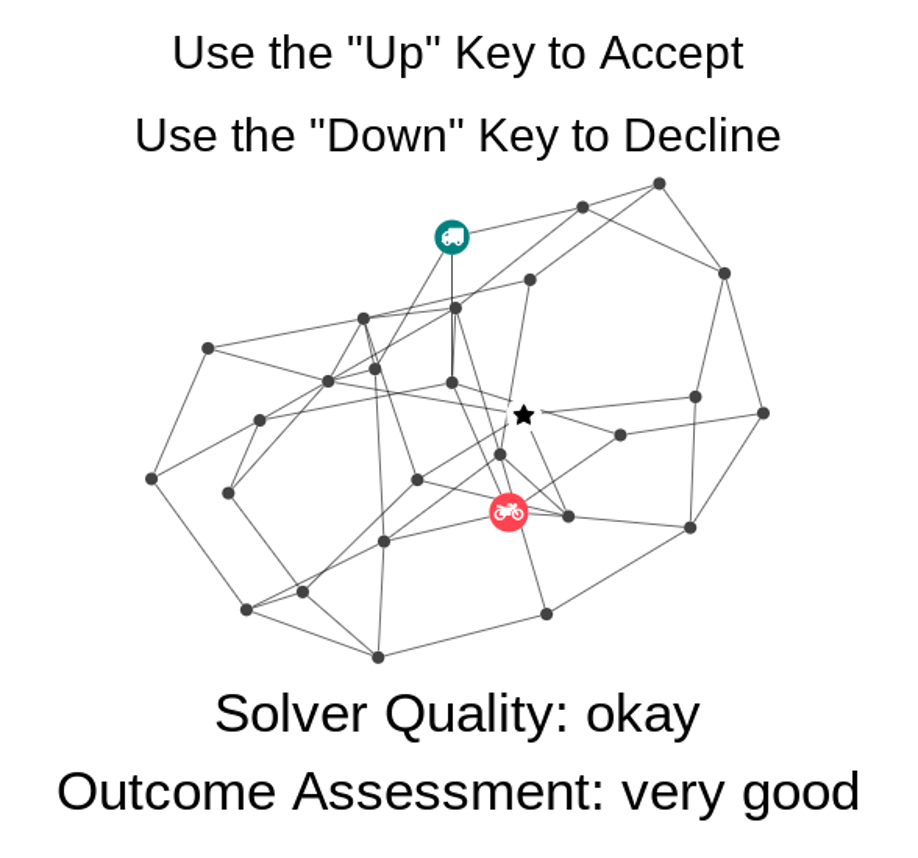
\includegraphics[width=0.45\linewidth]{Figures/experiment_screenshot_Compressed.png}
    \caption{Example screenshot from the Amazon Mechanical Turk experiment.} 
    \label{fig:experiment_screenshot}
\end{figure}

\begin{figure}[tbp]
    \centering
    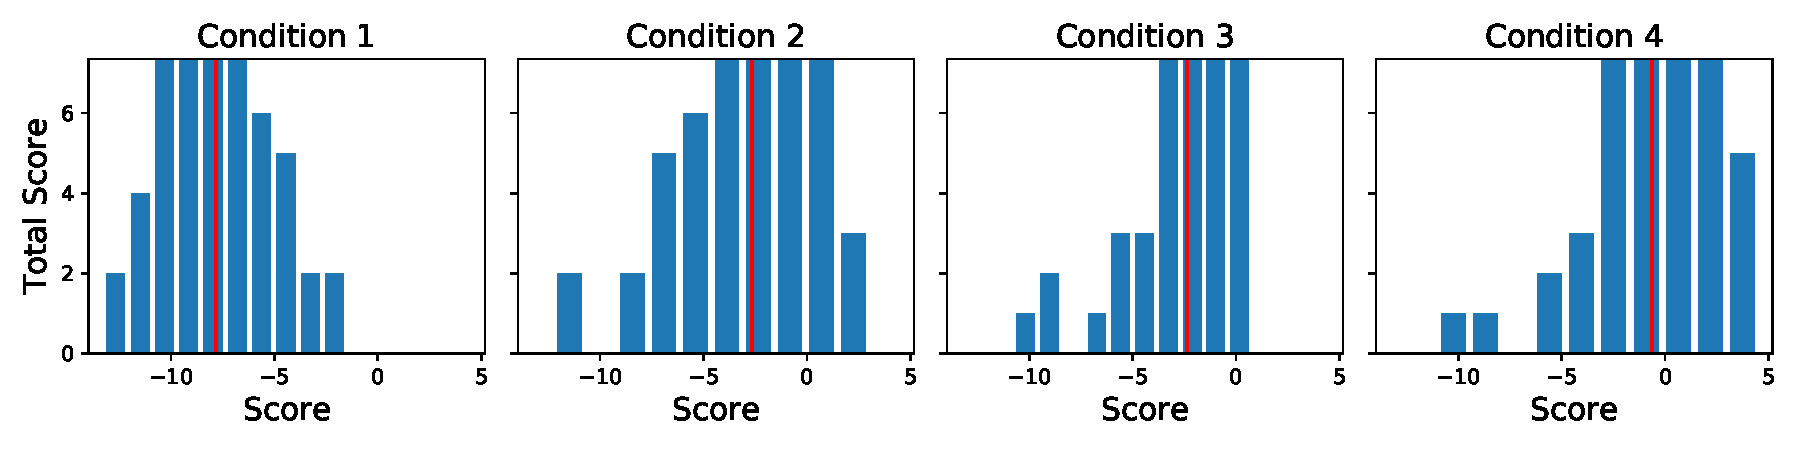
\includegraphics[width=1.0\linewidth]{Figures/total_score.pdf}
    \caption{Histogram of the Total Score from each condition. Red vertical lines indicate the sample mean.}
    \label{fig:total_score}
\end{figure}

At the end of the experiment participants answered survey questions about their perception of the ADT, how much they trusted the system, and how capable they thought it was. Our hypothesis is that the presence of self-confidence metrics would also affect these responses, but these data are still being analyzed.
